% Provenance (never printed): see sources/outline_sources.md (Year 3:
% facies analysis, depositional models, Walther's law, well logs). Brief:
% sources/book5/BRIEFS.md, ch. 17. Curves from figdata/bachelor-3/well_logs.py
% (unit tops from figdata/shared/region.py). Exercise and problem values in
% the Book 5 scratch calculator calc/ch17.py. The well Varden-2, its logs and
% the channel architecture of its sandstone are invented.
\chapter{Modelos de facies}\label{ch:b3:facies-models}

Un testigo de un sondeo de un kilómetro de profundidad: un metro de arena gruesa
con estratificación cruzada que descansa sobre una base neta y que se afina hacia
arriba hasta limo con huellas de raíces, y luego de nuevo arena sobre otra base neta.
El geólogo lee un río que serpenteó por su llanura, aunque ningún río corre allí
ahora. La lectura se apoya en dos herramientas: un conjunto de modelos, cada uno
un resumen de numerosos ejemplos modernos y antiguos de un mismo ambiente, y una
ley que convierte una sucesión vertical de capas en un mapa de los ambientes vecinos.

\begin{recall}
Las facies sedimentarias, el ambiente de depósito, las formas de lecho y la
estratificación cruzada, los deltas de los tres tipos, las corrientes de turbidez,
las turbiditas y los estratos gradados se tratan en el volumen de primer año, en su
capítulo sobre sedimentos clásticos y sus ambientes; la fábrica carbonatada, los arrecifes
y las plataformas carbonatadas se tratan en su capítulo sobre sedimentos carbonatados,
silíceos y evaporíticos; el registro de sondeo y la correlación de registros se tratan
en su capítulo sobre cortes geológicos. La porosidad y la permeabilidad están en los
libros de la escuela. Las \omterm{def:b3:sequence-stratigraphy:parasequence}{parasecuencias}, las \omterm{def:b3:sequence-stratigraphy:parasequence}{superficies de inundación} y los \omterm{def:b3:sequence-stratigraphy:tract}{cortejos sedimentarios}
están en el capítulo~\ref{ch:b3:sequence-stratigraphy}. Las olas en aguas profundas, cuyo movimiento se atenúa con la profundidad, están en los libros de física.
\end{recall}

\section{Facies, sucesiones y ley de Walther}\label{sec:b3:facies-models:walther}

Una facies sedimentaria se describe a partir de lo que puede verse en un testigo o en
un acantilado: tamaño de grano, selección, estructuras, fósiles, color. Una sola facies
rara vez es diagnóstica: la arena con estratificación cruzada se forma en ríos, en playas,
en canales mareales y en desiertos. Lo que identifica a un ambiente es el conjunto de
facies con las que se asocia y el orden en que las facies se suceden unas a otras.

\begin{definition}[Asociación de facies y sucesión de facies]\label{def:b3:facies-models:association}
Una \emph{asociación de facies}\index{asociación de facies} es un grupo de facies
que aparecen juntas y se depositaron en un mismo ambiente, como arena de canal,
limo de dique y lodo de llanura de inundación con raíces. Una \emph{sucesión de
facies}\index{sucesión de facies} es una secuencia vertical de facies en la que
alguna propiedad cambia de forma progresiva hacia arriba; en una \emph{sucesión
granodecreciente}\index{sucesión granodecreciente} el tamaño de grano disminuye hacia arriba,
y en una \emph{sucesión granocreciente}\index{sucesión granocreciente}
aumenta.
\end{definition}

\begin{definition}[Modelo de facies]\label{def:b3:facies-models:model}
Un \emph{modelo de facies}\index{modelo de facies} es un resumen general de un ambiente
de depósito, extraído de numerosos ejemplos modernos y antiguos: las facies que produce,
su geometría, sus relaciones laterales y las sucesiones que construye. Sirve como norma
con la que comparar un nuevo ejemplo, como
guía para observaciones posteriores, como predictor en situaciones nuevas y como base para
interpretar el ambiente.
\end{definition}

La relación entre lo lateral y lo vertical la establece una ley. Los ambientes vecinos
se encuentran uno junto a otro en cualquier momento: la playa junto a la \omterm{def:b3:facies-models:shoreface}{anteplaya}, la
\omterm{def:b3:facies-models:shoreface}{anteplaya} junto al lodo de plataforma externa. Cuando la línea de costa se desplaza,
cada ambiente acaba situándose sobre su vecino.

\begin{theorem}[Ley de Walther]\label{thm:b3:facies-models:walther}
En una sucesión concordante, sin una interrupción significativa de la sedimentación ni una
superficie erosiva, las facies que se superponen directamente se depositaron en ambientes
que, en su momento, estaban situados uno junto a otro.
\end{theorem}

\begin{proof}
Considérense cinturones de ambientes, cada uno una franja paralela a la línea de costa,
que migran conjuntamente a través de la cuenca mientras el fondo subside o el nivel del
mar sube. En un lugar fijo, los cinturones pasan uno tras otro, en el orden en que
estaban situados uno junto a otro, y cada uno deja su depósito encima del depósito del
cinturón que lo precedió. Si la sedimentación es continua, el orden vertical de los
depósitos es, por tanto, el orden lateral de los cinturones. Una interrupción o una
superficie de erosión rompe el argumento: los cinturones que pasaron durante el hiato
no dejaron nada, o sus depósitos fueron eliminados, y facies de ambientes no adyacentes
entran en contacto.
\end{proof}

\begin{omfigure}
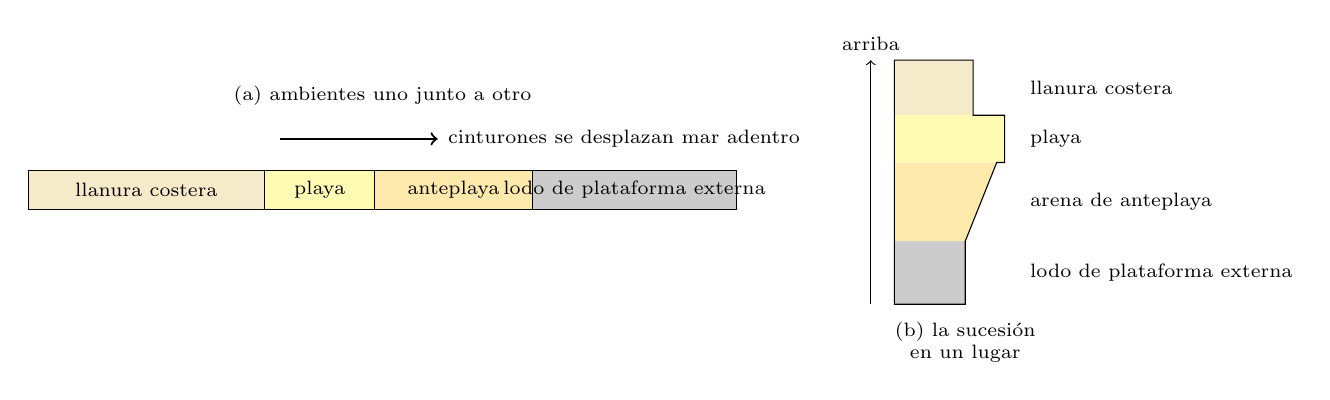
\begin{tikzpicture}[font=\scriptsize, x=1cm, y=1cm]
% environments side by side, with a shoreline that moves seaward
\fill[yellow!35!brown!25] (0,0) rectangle (3,0.5);
\fill[yellow!30] (3,0) rectangle (4.4,0.5);
\fill[yellow!50!orange!30] (4.4,0) rectangle (6.4,0.5);
\fill[black!20] (6.4,0) rectangle (9,0.5);
\draw (0,0) rectangle (9,0.5);
\foreach \x in {3,4.4,6.4} {\draw (\x,0) -- (\x,0.5);}
\node at (1.5,0.25) {llanura costera};
\node at (3.7,0.25) {playa};
\node at (5.4,0.25) {anteplaya};
\node at (7.7,0.25) {lodo de plataforma externa};
\draw[->, thick] (3.2,0.9) -- (5.2,0.9) node[right] {cinturones se desplazan mar adentro};
\node[anchor=south] at (4.5,1.2) {(a) ambientes uno junto a otro};
% vertical succession at a place
\begin{scope}[xshift=11cm, yshift=-1.2cm]
\fill[black!20] (0,0) rectangle (0.9,0.8);
\fill[yellow!50!orange!30] (0,0.8) -- (0.9,0.8) -- (1.3,1.8) -- (0,1.8) -- cycle;
\fill[yellow!30] (0,1.8) rectangle (1.4,2.4);
\fill[yellow!35!brown!25] (0,2.4) rectangle (1.0,3.1);
\draw (0,0) -- (0.9,0) -- (0.9,0.8) -- (1.3,1.8) -- (1.4,1.8) -- (1.4,2.4) -- (1.0,2.4) -- (1.0,3.1) -- (0,3.1) -- cycle;
\node[anchor=west] at (1.6,0.4) {lodo de plataforma externa};
\node[anchor=west] at (1.6,1.3) {arena de anteplaya};
\node[anchor=west] at (1.6,2.1) {playa};
\node[anchor=west] at (1.6,2.75) {llanura costera};
\draw[->] (-0.3,0) -- (-0.3,3.1) node[above] {arriba};
\node[anchor=north, align=center] at (0.9,-0.1) {(b) la sucesión\\ en un lugar};
\end{scope}
\end{tikzpicture}

\par\smallskip{\small La ley de Walther. (a) Los ambientes se disponen uno junto a otro a lo largo
de un perfil; (b) a medida que las franjas se desplazan hacia mar adentro, un lugar recibe lodo de plataforma externa,
después arena de \omterm{def:b3:facies-models:shoreface}{anteplaya}, arena de playa y depósitos de llanura costera: una
\omterm{def:b3:facies-models:association}{sucesión granocreciente} en el orden de las franjas (la anchura en el registro
indica grano más grueso).}\label{fig:b3:facies-models:walther}
\end{omfigure}

La ley funciona en ambos sentidos. Una regresión apila las franjas en su orden de mar adentro
hacia arriba, y una transgresión lo hace en orden inverso; y una sucesión vertical leída
en un testigo ofrece el mapa de los ambientes vecinos en aquel momento. La ley falla
justo donde el capítulo~\ref{ch:b3:sequence-stratigraphy} sitúa sus superficies clave:
a través de un \omterm{def:b3:sequence-stratigraphy:sequence}{límite de secuencia}, donde la exposición y la erosión depositan arena fluvial sobre
lodo de plataforma, y en una \omterm{def:b3:sequence-stratigraphy:parasequence}{superficie de inundación}, donde el lodo de plataforma externa yace directamente sobre
la llanura costera.

\section{Ríos}\label{sec:b3:facies-models:rivers}

\begin{definition}[Ríos trenzados y meandriformes]\label{def:b3:facies-models:rivers}
Un \emph{río trenzado}\index{río trenzado} discurre por varios canales someros
que se dividen y se reúnen alrededor de barras, sobre una llanura empinada con abundante
carga gruesa y caudal variable. Un \emph{río meandriforme}\index{río meandriforme}
discurre por un único canal sinuoso sobre una llanura más suave, y transporta más
sedimento fino; migra erosionando la orilla externa de cada meandro y
depositando en la interna. El depósito de la orilla interna es una \emph{barra
de meandro}\index{barra de meandro}. La \emph{avulsión}\index{avulsión} es el abandono de
un canal por un nuevo cauce a través de la llanura de inundación, por lo general
tras una crecida que rompe un dique natural.
\end{definition}

Una \omterm{def:b3:facies-models:rivers}{barra de meandro} crece lateralmente a medida que migra el meandro, de modo que en cualquier punto registra
la sección transversal del canal, de abajo arriba: un depósito residual de los clastos más
gruesos sobre una base erosiva, arena con estratificación cruzada de las dunas del canal profundo,
arena más fina con rizos del techo somero de la barra y, después, el
limo y el lodo de la llanura de inundación con raíces y suelos. Según la ley de Walther, esta
\omterm{def:b3:facies-models:association}{sucesión granodecreciente}, de pocos metros de espesor, tiene el espesor de la
profundidad del canal. Un \omterm{def:b3:facies-models:rivers}{río trenzado} deja mantos apilados de arena con estratificación cruzada
y grava con poco lodo, cuyo tamaño de grano apenas cambia hacia arriba; sus finos
son arrastrados. La \omterm{def:b3:facies-models:rivers}{avulsión} desplaza el cinturón de canales por la llanura, de modo que
los cuerpos de canal se apilan al azar entre lodos de llanura de inundación,
separados por bases erosivas netas.

\begin{omfigure}
\begin{tikzpicture}[font=\scriptsize, x=1cm, y=1cm]
% (a) braided plan
\begin{scope}
\fill[yellow!35!brown!20] (0,0) rectangle (4.6,2.4);
\draw[omDef!60, line width=1.6pt] (0,1.2) .. controls (0.8,1.6) and (1.4,0.6) .. (2.3,1.0) .. controls (3.0,1.3) and (3.6,0.7) .. (4.6,1.0);
\draw[omDef!60, line width=1.6pt] (0,1.2) .. controls (0.8,0.8) and (1.6,1.9) .. (2.4,1.6) .. controls (3.2,1.3) and (3.8,1.9) .. (4.6,1.6);
\draw[omDef!60, line width=1.2pt] (1.2,1.25) .. controls (1.8,1.5) and (2.6,1.2) .. (3.3,1.35);
\fill[yellow!45] (1.5,1.15) ellipse (0.35 and 0.12);
\fill[yellow!45] (3.0,1.25) ellipse (0.4 and 0.12);
\node[anchor=south] at (2.3,2.45) {(a) trenzado};
\end{scope}
% (b) meandering plan
\begin{scope}[xshift=5.4cm]
\fill[green!30!black!12] (0,0) rectangle (4.6,2.4);
\draw[omDef!60, line width=2pt] (0,1.2) .. controls (0.6,2.2) and (1.4,2.2) .. (1.6,1.2) .. controls (1.8,0.2) and (2.8,0.2) .. (3.0,1.2) .. controls (3.2,2.2) and (4.0,2.2) .. (4.6,1.2);
\fill[yellow!45] (0.8,1.45) ellipse (0.3 and 0.2);
\fill[yellow!45] (2.3,0.95) ellipse (0.3 and 0.2);
\fill[yellow!45] (3.8,1.45) ellipse (0.3 and 0.2);
\node at (2.3,0.95) {bm};
\draw[omDef!40, line width=1pt, densely dashed] (0.4,0.2) .. controls (1.0,0.7) and (1.6,0.4) .. (2.0,0.1);
\node[anchor=west, font=\tiny] at (2.6,2.15) {llanura de inundación};
\node[anchor=south] at (2.3,2.45) {(b) meandriforme};
\end{scope}
% logs
\begin{scope}[xshift=10.8cm]
\fill[yellow!45] (0,0) -- (1.2,0) -- (1.2,2.0) -- (0,2.0) -- cycle;
\draw (0,0) -- (1.2,0) -- (1.15,0.6) -- (1.2,0.65) -- (1.1,1.3) -- (1.2,1.35) -- (1.15,2.0) -- (0,2.0) -- cycle;
\node[anchor=north] at (0.6,-0.05) {trenzado};
\end{scope}
\begin{scope}[xshift=12.6cm]
\fill[yellow!45] (0,0) -- (1.2,0) -- (1.1,0.9) -- (0.45,1.6) -- (0,1.6) -- cycle;
\fill[green!30!black!15] (0,1.6) rectangle (0.3,2.2);
\draw (0,0) -- (1.2,0) -- (1.1,0.9) -- (0.45,1.6) -- (0.3,1.6) -- (0.3,2.2) -- (0,2.2) -- cycle;
\draw[decorate, decoration={snake, amplitude=0.4mm, segment length=1.5mm}] (0,0) -- (1.2,0);
\node[anchor=north] at (0.6,-0.05) {barra de meandro};
\node[anchor=west, font=\tiny] at (0.35,1.9) {raíces};
\end{scope}
\end{tikzpicture}

\par\smallskip{\small (a) Un \omterm{def:b3:facies-models:rivers}{río trenzado}: varios canales alrededor de barras de
arena y grava. (b) Un \omterm{def:b3:facies-models:rivers}{río meandriforme}: un único canal sinuoso, \omterm{def:b3:facies-models:rivers}{barras de meandro} (bm)
en las orillas internas, un antiguo cauce (discontinuo) abandonado por \omterm{def:b3:facies-models:rivers}{avulsión}. A la derecha:
registros granulométricos de los depósitos (la anchura indica grano más grueso): mantos de arena apilados
con poco cambio hacia arriba para el \omterm{def:b3:facies-models:rivers}{río trenzado}, una \omterm{def:b3:facies-models:association}{sucesión granodecreciente} de base neta
coronada por lodo de llanura de inundación con raíces para la \omterm{def:b3:facies-models:rivers}{barra de
meandro}.}\label{fig:b3:facies-models:rivers}
\end{omfigure}

\section{Líneas de costa, deltas y plataformas}\label{sec:b3:facies-models:shelves}

Los deltas del volumen de primer año, dominados por ríos, oleaje o mareas, todos
progradan por el mismo mecanismo: la desembocadura deposita su carga donde la
corriente se frena, y el frente deltaico progresa sobre sus propios lodos de prodelta. Un
frente deltaico o de \omterm{def:b3:facies-models:shoreface}{anteplaya} progradante deja, según la ley de Walther, una
\omterm{def:b3:facies-models:association}{sucesión granocreciente}: lodo de plataforma externa, alternancias de lodo y arena de tormenta,
arena de \omterm{def:b3:facies-models:shoreface}{anteplaya} y playa. Cada \omterm{def:b3:sequence-stratigraphy:parasequence}{parasecuencia} del capítulo anterior es una de estas
sucesiones.

\begin{definition}[Anteplaya y niveles de base del oleaje]\label{def:b3:facies-models:shoreface}
La \emph{anteplaya}\index{anteplaya} es la zona en pendiente situada mar adentro de la
playa, donde el oleaje retrabaja de forma continua el fondo marino. Su base es el
\emph{nivel de base del oleaje de buen tiempo}\index{nivel de base del oleaje de buen tiempo}, la profundidad
por debajo de la cual el oleaje ordinario ya no mueve el sedimento del fondo. El \emph{nivel de base del
oleaje de tormenta}\index{nivel de base del oleaje de tormenta} es el límite más profundo alcanzado por el oleaje de tormenta;
entre ambos, el lodo se deposita con tiempo tranquilo y se retrabaja en capas de arena
durante las tormentas. Por debajo del nivel de base del oleaje de tormenta, el fondo no se ve perturbado por el oleaje.
\end{definition}

\begin{omfigure}
\begin{tikzpicture}[font=\scriptsize, x=1cm, y=1.6cm]
\fill[omSea!60] (0,2.2) -- (13,2.2) -- (13,0.2) -- (5.5,0.9) -- (2.0,1.9) -- (0.6,2.2) -- cycle;
\fill[yellow!40] (0,2.4) -- (0.6,2.2) -- (2.0,1.9) -- (5.5,0.9) -- (5.5,0.0) -- (0,0.0) -- cycle;
\fill[black!18] (5.5,0.9) -- (13,0.2) -- (13,0) -- (5.5,0) -- cycle;
\draw[thick] (0,2.4) -- (0.6,2.2) -- (2.0,1.9) -- (5.5,0.9) -- (13,0.2);
\draw[omDef] (0,2.2) -- (13,2.2);
\draw[omDef, densely dashed] (1.6,1.97) -- (13,1.97);
\draw[omDef, densely dashed] (5.5,0.9) -- (13,0.9);
\node[omDef, anchor=north west] at (9.3,1.95) {nivel de base del oleaje de buen tiempo};
\node[omDef, anchor=north west] at (9.3,0.88) {nivel de base del oleaje de tormenta};
\node[anchor=south] at (0.5,2.42) {playa};
\node at (1.8,1.35) {anteplaya};
\node at (4.3,0.45) {transición mar adentro};
\node at (9.0,0.15) {lodo de plataforma externa};
\node[align=center] at (7.4,1.45) {capas de arena de tormenta,\\ estratificación cruzada hummocky};
\end{tikzpicture}

\par\smallskip{\small Perfil de línea de costa dominada por el oleaje (esquemático, escala vertical
muy exagerada). Por encima del \omterm{def:b3:facies-models:shoreface}{nivel de base del oleaje de buen tiempo}, la arena de la \omterm{def:b3:facies-models:shoreface}{anteplaya}
se retrabaja a diario; entre ambos niveles de base, el lodo alterna con capas de arena
depositadas por tormentas; por debajo del \omterm{def:b3:facies-models:shoreface}{nivel de base del oleaje de tormenta} se
acumula lodo.}\label{fig:b3:facies-models:shoreface}
\end{omfigure}

El movimiento orbital de una onda en aguas profundas se atenúa como $e^{-2\pi z/\lambda}$
con la profundidad $z$, para una longitud de onda $\lambda$: a media longitud de onda conserva el
\qty{4}{\percent} de su amplitud en superficie, lo que fija la escala de un
nivel de base del oleaje. Los registros de boyas de más de dos millones de espectros de oleaje del Caribe, el golfo de México y el Atlántico occidental
dan longitudes de onda modales de unos
\qty{75}{m} en los mares protegidos y de unos \qty{110}{m} en el margen abierto,
y muestran que, promediadas durante semanas o años, las longitudes de onda no se separan en
una clase de buen tiempo y otra de tormenta: la probabilidad de que una onda remueva el fondo
aumenta de forma continua a medida que el agua se hace más somera. Los dos niveles de base del oleaje siguen siendo términos útiles
para zonas de un perfil, no profundidades precisas.
% ledger: losspeters10:wavebase

\begin{definition}[Estratificación cruzada hummocky]\label{def:b3:facies-models:hcs}
La \emph{estratificación cruzada hummocky}\index{estratificación cruzada hummocky} es
una estratificación de arena fina en láminas suavemente curvadas, cóncavas hacia arriba
(surcos) y convexas hacia arriba (montículos), que se cortan entre sí con ángulos bajos y
se engruesan y adelgazan lateralmente, con longitudes de onda de un metro a varios metros. Se forma
por los flujos oscilatorios y combinados del oleaje de tormenta, entre el \omterm{def:b3:facies-models:shoreface}{nivel de base del
oleaje de buen tiempo} y el \omterm{def:b3:facies-models:shoreface}{nivel de base del oleaje de tormenta}.
\end{definition}

\begin{inthefield}[Capas de tormenta en una plataforma silúrica]
\begin{minipage}[t]{0.42\linewidth}\vspace{0pt}
En la Formación Arisaig de Nueva Escocia, capas de arenisca fina separan
lutitas más oscuras. Los geólogos que han estudiado estas capas reconocen las láminas bajas, curvadas,
láminas que se cortan, propias de la \omterm{def:b3:facies-models:hcs}{estratificación cruzada hummocky}: cada capa registra una
tormenta que agitó la plataforma por debajo del alcance del oleaje cotidiano, y el lodo
que la rodea, la larga calma entre tormentas.
\end{minipage}\hfill
\begin{minipage}[t]{0.54\linewidth}\vspace{0pt}
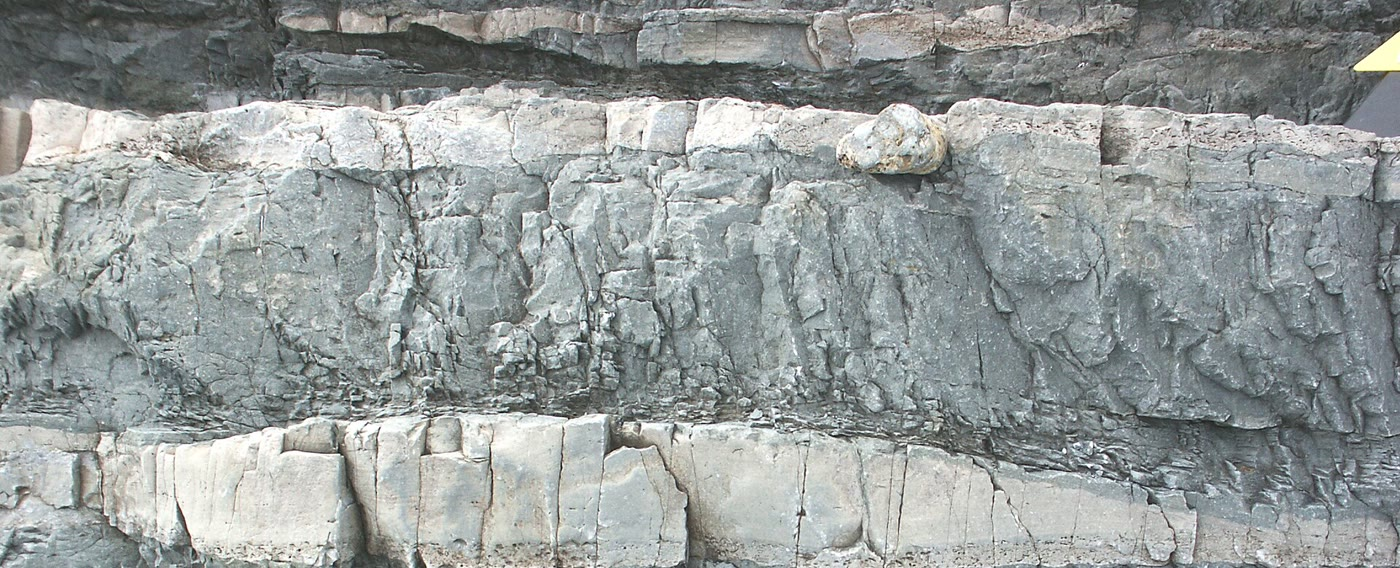
\includegraphics[width=\linewidth]{images/book5/b3-hummocky-cross-stratification.jpg}

{\scriptsize \omterm{def:b3:facies-models:hcs}{Estratificación cruzada hummocky} en la Formación Arisaig
(silúrica), cerca de Arisaig, Nueva Escocia. Fotografía: Michael C. Rygel, CC BY-SA 3.0
(recortada).}
\end{minipage}
\end{inthefield}
% ledger: photo:b3-hcs

Donde dominan las mareas, cambian las facies: las corrientes de flujo y reflujo construyen
estratificaciones cruzadas de sentido opuesto, los recubrimientos de lodo se depositan en cada estoa
y el espesor de los paquetes entre recubrimientos aumenta y disminuye con
el ciclo de mareas vivas y muertas. Los canales mareales, las llanuras de marea y las crestas de arena
tienen modelos propios, construidos de la misma manera.

\section{Aguas profundas}\label{sec:b3:facies-models:deep}

Una corriente de turbidez que se frena deposita su carga según el orden de sedimentación:
primero los granos más gruesos y por último los más finos. Una capa de turbidita completa muestra
este orden en cinco divisiones.

\begin{definition}[Secuencia de Bouma]\label{def:b3:facies-models:bouma}
La \emph{secuencia de Bouma}\index{secuencia de Bouma} es la sucesión ideal de
divisiones en una capa de turbidita, de la base a la cima: Ta, arena masiva o gradada sobre
una base erosiva con marcas de corriente y de herramienta; Tb, arena con laminación paralela; Tc,
arena fina con laminación cruzada de rizo y convoluta; Td, limo con laminación paralela;
Te, lodo, en parte procedente de la corriente de turbidez y en parte del lento asentamiento
entre flujos.
\end{definition}

Pocas capas muestran las cinco: cerca de la fuente la corriente es rápida y deja divisiones Ta gruesas
con las superiores erosionadas por el flujo siguiente; lejos de ella solo
llegan las divisiones más finas, de Tc a Te. La secuencia registra así la
pérdida de energía de un flujo, y el cambio de las capas a lo largo del abanico, la pérdida de energía de los flujos
con la distancia.

\begin{definition}[Abanico submarino]\label{def:b3:facies-models:fan}
Un \emph{abanico submarino}\index{abanico submarino} es un cono de sedimento al pie
de un talud continental, alimentado por un cañón: un abanico superior con un canal principal
entre diques naturales, un abanico medio de canales distributarios que terminan en lóbulos de arena,
y un abanico inferior de turbiditas delgadas que pasan a lodo de fondo de cuenca.
\end{definition}

A lo largo del margen, las corrientes profundas impulsadas por la circulación oceánica retrabajan el
sedimento fino del talud, dando lugar a contorritas, montículos y deriva de
limo y lodo bioturbados que crecen a lo largo de las isobatas y no pendiente abajo
talud.

\begin{omfigure}
\begin{tikzpicture}[font=\scriptsize, x=1cm, y=1cm]
% (a) Bouma log
\begin{scope}
\fill[yellow!45] (0,0) -- (1.6,0) -- (1.6,1.2) -- (0,1.2) -- cycle;
\fill[yellow!35] (0,1.2) rectangle (1.3,1.8);
\fill[yellow!25] (0,1.8) rectangle (1.0,2.4);
\fill[black!12] (0,2.4) rectangle (0.7,2.8);
\fill[black!25] (0,2.8) rectangle (0.4,3.3);
\draw (0,0) -- (1.6,0) -- (1.6,1.2) -- (1.3,1.2) -- (1.3,1.8) -- (1.0,1.8) -- (1.0,2.4) -- (0.7,2.4) -- (0.7,2.8) -- (0.4,2.8) -- (0.4,3.3) -- (0,3.3) -- cycle;
\draw[decorate, decoration={snake, amplitude=0.5mm, segment length=2mm}] (0,0) -- (1.6,0);
\foreach \y in {1.35,1.5,1.65} {\draw[black!60] (0.05,\y) -- (1.25,\y);}
\foreach \x in {0.15,0.45,0.75} {\draw[black!60] (\x,1.95) .. controls (\x+0.08,2.1) .. (\x+0.2,1.95);}
\foreach \y in {2.5,2.6,2.7} {\draw[black!60] (0.05,\y) -- (0.65,\y);}
\foreach \y/\t in {0.6/Ta, 1.5/Tb, 2.1/Tc, 2.6/Td, 3.05/Te} {\node[anchor=west] at (1.9,\y) {\t};}
\node[anchor=west, align=left, font=\tiny] at (2.4,0.6) {arena gradada o masiva,\\ base erosiva};
\node[anchor=west, font=\tiny] at (2.4,1.5) {laminación paralela};
\node[anchor=west, font=\tiny] at (2.4,2.1) {rizos, laminación convoluta};
\node[anchor=west, font=\tiny] at (2.4,2.6) {limo laminado};
\node[anchor=west, font=\tiny] at (2.4,3.05) {lodo};
\node[anchor=north] at (1.6,-0.15) {(a) una capa de turbidita};
\end{scope}
% (b) fan plan
\begin{scope}[xshift=8.2cm, yshift=0.2cm]
\fill[black!8] (-1.0,-0.2) rectangle (5.6,3.1);
\fill[yellow!20] (0.3,2.9) .. controls (1.6,2.6) and (4.9,2.0) .. (5.2,0.9) .. controls (4.6,-0.1) and (1.2,0.1) .. (0.3,1.6) -- cycle;
\fill[yellow!45] (1.9,1.9) ellipse (0.55 and 0.3);
\fill[yellow!45] (2.6,1.0) ellipse (0.55 and 0.3);
\fill[yellow!45] (3.4,1.75) ellipse (0.5 and 0.28);
\draw[omDef, line width=1.4pt] (-0.9,3.0) .. controls (-0.3,2.8) and (0.4,2.6) .. (1.0,2.2);
\draw[omDef, line width=0.8pt] (1.0,2.2) -- (1.6,1.95);
\draw[omDef, line width=0.8pt] (1.0,2.2) -- (2.3,1.15);
\draw[omDef, line width=0.8pt] (1.0,2.2) .. controls (2.0,2.4) .. (3.1,1.85);
\node[anchor=south west] at (-0.95,3.0) {cañón};
\node[anchor=east] at (0.55,2.0) {diques naturales};
\node[align=center, font=\tiny] at (2.6,1.0) {lóbulo};
\node at (4.4,0.7) {abanico inferior};
\node[black!60] at (4.9,2.85) {fondo de cuenca};
\node[anchor=north] at (2.3,-0.25) {(b) un abanico submarino en planta};
\end{scope}
\end{tikzpicture}

\par\smallskip{\small (a) La \omterm{def:b3:facies-models:bouma}{secuencia de Bouma} de una capa turbidítica completa,
dibujada como perfil granulométrico (la anchura indica mayor tamaño de grano), con sus cinco divisiones. (b)
Un \omterm{def:b3:facies-models:fan}{abanico submarino} en planta: un cañón alimenta un canal entre diques naturales, que
se divide en canales distributarios que terminan en lóbulos de arena; capas finas de turbiditas
se extienden sobre el abanico inferior.}\label{fig:b3:facies-models:deep}
\end{omfigure}

\section{Plataformas carbonatadas}\label{sec:b3:facies-models:carbonates}

El sedimento carbonatado se forma en el lugar donde se encuentra, por la acción de organismos en aguas cálidas, claras
y poco profundas, y sus facies siguen el perfil de la plataforma que la
fábrica carbonatada construye para sí misma.

\begin{definition}[Rampa carbonatada y plataforma bordeada]\label{def:b3:facies-models:ramp}
Una \emph{rampa carbonatada}\index{rampa carbonatada} es una plataforma cuyo fondo
desciende suave y uniformemente desde la línea de costa hacia la cuenca, sin ruptura:
sus cinturones de facies, desde planicies de marea y arenas de barrera de playa hasta granos de bajío,
arena bioclástica y lodo calcáreo de mar abierto, son amplios y pasan gradualmente unos a otros,
clasificados por la energía del oleaje, que disminuye con la profundidad. Una \emph{plataforma
bordeada}\index{plataforma bordeada} es una plataforma de cima plana con una marcada ruptura
de pendiente en su margen, donde arrecifes y bajíos arenosos construyen un borde que protege
una laguna situada detrás; más allá del borde, una pendiente abrupta vierte bloques y granos
hacia la cuenca.
\end{definition}

\begin{omfigure}
\begin{tikzpicture}[font=\scriptsize, x=1cm, y=1cm]
\begin{scope}
\fill[omSea!60] (0,1.6) -- (6.4,1.6) -- (6.4,0.3) -- cycle;
\fill[black!10] (0,1.6) -- (6.4,0.3) -- (6.4,0) -- (0,0) -- cycle;
\draw[thick] (0,1.7) -- (0.3,1.6) -- (6.4,0.3);
\draw[omDef] (0,1.6) -- (6.4,1.6);
\node[anchor=south] at (0.6,1.65) {planicie de marea};
\node[rotate=-12, font=\tiny] at (1.5,1.08) {granos de bajío};
\node[rotate=-12, font=\tiny] at (3.4,0.66) {arena bioclástica};
\node[rotate=-12, font=\tiny] at (5.3,0.26) {lodo calcáreo};
\node[anchor=north, align=center] at (3.2,-0.1) {(a) rampa: pendiente uniforme,\\ cinturones graduales};
\end{scope}
\begin{scope}[xshift=7.2cm]
\fill[omSea!60] (0,1.6) -- (6.4,1.6) -- (6.4,0.2) -- (4.4,0.3) -- (3.6,1.55) -- (3.2,1.6) -- (0.3,1.6) -- cycle;
\fill[omSea!60] (0.3,1.6) -- (3.2,1.6) -- (3.0,1.35) -- (0.6,1.35) -- cycle;
\fill[black!10] (0,1.7) -- (0.3,1.6) -- (0.6,1.35) -- (3.0,1.35) -- (3.2,1.6) -- (3.6,1.55) -- (4.4,0.3) -- (6.4,0.2) -- (6.4,0) -- (0,0) -- cycle;
\draw[thick] (0,1.7) -- (0.3,1.6) -- (0.6,1.35) -- (3.0,1.35) -- (3.2,1.6) -- (3.6,1.55) -- (4.4,0.3) -- (6.4,0.2);
\fill[orange!50] (3.05,1.4) -- (3.2,1.6) -- (3.55,1.56) -- (3.6,1.4) -- cycle;
\draw[omDef] (0,1.6) -- (6.4,1.6);
\node at (1.8,1.12) {laguna};
\node[anchor=south] at (3.35,1.65) {borde arrecifal};
\node[anchor=west] at (4.2,0.95) {pendiente abrupta};
\node at (5.5,0.6) {cuenca};
\node[anchor=north, align=center] at (3.2,-0.1) {(b) plataforma bordeada: un borde,\\ una laguna, una pendiente};
\end{scope}
\end{tikzpicture}

\par\smallskip{\small Perfiles esquemáticos de plataformas carbonatadas (esquemáticos, con escala
vertical muy exagerada). (a) Una rampa: cinturones ordenados por la energía del oleaje a lo largo de una
pendiente uniforme. (b) Una \omterm{def:b3:facies-models:ramp}{plataforma bordeada}: un arrecife y un borde de bajíos en la ruptura
de pendiente protege una laguna de lodo calcáreo; la pendiente más allá recibe bloques y granos
desprendidos del borde.}\label{fig:b3:facies-models:platforms}
\end{omfigure}

Sobre la cima de una plataforma plana, una pequeña subida del nivel relativo del mar inunda las
planicies de marea, y la fábrica, que trabaja más rápido en el agua más somera, rellena de nuevo
el espacio hasta el nivel del mar en poco tiempo. El resultado es una sucesión de ciclos
perimareales de un metro o pocos metros de espesor, cada uno una \omterm{def:b3:sequence-stratigraphy:parasequence}{parasecuencia} de somerización
hacia arriba, desde lodo submareal hasta una planicie de marea con grietas de desecación o tapetes
microbianos, coronada por la siguiente \omterm{def:b3:sequence-stratigraphy:parasequence}{superficie de inundación}.

\section{Testigos y registros de pozo}\label{sec:b3:facies-models:logs}

La mayor parte de la roca situada bajo las cuencas sedimentarias se conoce a partir de sondeos. Unos pocos
se testifican, y sus testigos se describen capa a capa como si fueran un acantilado; casi todos
se registran.

\begin{definition}[Registros de pozo]\label{def:b3:facies-models:wireline}
Un \emph{registro de pozo}\index{registro de pozo} es un registro continuo de una
propiedad física de las rocas en función de la profundidad, medida por una sonda descendida
mediante un cable en un sondeo. El \emph{registro de rayos gamma}\index{registro de rayos gamma}
registra la radiación gamma natural de la roca, en unidades API: alta en
lutita, cuyas arcillas retienen potasio, torio y uranio, y baja en
arena cuarzosa limpia y en caliza. El \emph{registro de densidad}\index{registro de densidad}
registra la densidad aparente a partir de la dispersión de los rayos gamma emitidos por una
fuente situada en la sonda. El \emph{registro sónico}\index{registro sónico} registra el
tiempo de tránsito por intervalo de una onda compresional, en microsegundos por pie. El
\emph{registro de neutrones}\index{registro de neutrones} registra la pérdida de velocidad de los neutrones
por el hidrógeno, y por tanto el agua retenida en los poros y en las arcillas.
\end{definition}
% ledger: keys:gamma, keys:density-porosity, keys:sonic

La unidad API de rayos gamma se define en una fosa de calibración: una doscientosava parte de la
diferencia entre una zona de radiactividad despreciable y una zona con
los radioisótopos de una lutita media a aproximadamente el doble de su concentración. El carbón,
la caliza y la dolomía suelen ser menos radiactivos que la lutita; la arenisca cuarzosa es baja, y una
arcosa rica en feldespato potásico, más alta; cualquier roca puede hacerse radiactiva por el uranio
transportado por el agua subterránea.
% ledger: keys:gamma

\begin{proposition}[Porosidad a partir de la densidad y el tiempo de tránsito]\label{prop:b3:facies-models:porosity}
Una roca de porosidad $\phi$, con granos de densidad $\rho_{\mathrm{ma}}$ y
poros rellenos de un fluido de densidad $\rho_f$, tiene la densidad aparente
$\rho_b = (1 - \phi)\rho_{\mathrm{ma}} + \phi\rho_f$, de modo que
\[
\phi = \frac{\rho_{\mathrm{ma}} - \rho_b}{\rho_{\mathrm{ma}} - \rho_f}.
\]
Si una onda compresional atraviesa los granos y el fluido en serie, en
longitudes proporcionales a $1 - \phi$ y $\phi$, su tiempo de tránsito es
$\Delta t = (1 - \phi)\Delta t_{\mathrm{ma}} + \phi\Delta t_f$ (la
ecuación del promedio temporal), y $\phi = (\Delta t - \Delta
t_{\mathrm{ma}})/(\Delta t_f - \Delta t_{\mathrm{ma}})$.
\end{proposition}

\begin{proof}
Una unidad de volumen de roca contiene un volumen $1 - \phi$ de granos y $\phi$ de
fluido; su masa es $(1 - \phi)\rho_{\mathrm{ma}} + \phi\rho_f$, de donde se despeja
$\phi$. Para la onda, un camino de longitud unidad atraviesa $1 - \phi$ de
granos y $\phi$ de fluido, y los tiempos se suman.
\end{proof}

Las densidades de los granos son \qty{2.65}{g/cm^3} para el cuarzo y \qty{2.71}{g/cm^3} para
la caliza; el agua de poro tiene \qty{1.0}{g/cm^3} cuando es dulce y hasta
\qty{1.1}{g/cm^3} como salmuera. Los tiempos de tránsito van de 42 a
\qty{48}{\micro\second/ft} en la dolomía, de 48 a 53 en la caliza, 53 en una arenisca
consolidada, y 189 en salmuera. La ecuación de la densidad es exacta para
una matriz conocida; la ecuación del promedio temporal es una regla empírica que funciona
mejor en rocas consolidadas con poros intergranulares. Las lutitas incumplen ambas:
las arcillas tienen sus propias densidades y retienen agua ligada.
% ledger: keys:density-porosity, keys:sonic

\begin{definition}[Razón neto--bruto]\label{def:b3:facies-models:ntg}
La \emph{razón neto--bruto}\index{razón neto--bruto} de un intervalo es el
espesor de su roca de calidad de yacimiento, normalmente arena identificada en el
\omterm{def:b3:facies-models:wireline}{registro de rayos gamma} por debajo de un valor de corte, dividido entre el espesor total del intervalo.
\end{definition}

La forma de la curva de rayos gamma a través de un cuerpo arenoso es una herramienta de facies.
Una \emph{campana}, limpia en la base y más arcillosa hacia arriba, es una \omterm{def:b3:facies-models:association}{sucesión granodecreciente},
como en una \omterm{def:b3:facies-models:rivers}{barra de meandro} o en el relleno de un canal; un \emph{embudo}, arcilloso en
la base y limpio en el techo, una \omterm{def:b3:facies-models:association}{sucesión granocreciente}, como en una
\omterm{def:b3:facies-models:shoreface}{anteplaya} progradante o frente deltaico; un \emph{cilindro}, limpio en toda su extensión y con
límites netos, una arena apilada de \omterm{def:b3:facies-models:rivers}{río trenzado}, una duna eólica o un
banco carbonatado. Las formas son indicios, no pruebas: un testigo, o al menos los
registros vecinos, deben confirmarlas.

\begin{omfigure}
\begin{tikzpicture}
\begin{groupplot}[group style={group size=3 by 1, horizontal sep=0.2cm,
    y descriptions at=edge left},
  omrecord, y dir=reverse, ymin=700, ymax=1200, width=0.28\linewidth,
  height=0.62\linewidth, ytick={700,800,900,1000,1100,1200},
  tick label style={font=\scriptsize}, label style={font=\small},
  xlabel style={font=\small}]
\nextgroupplot[xlabel={GR (API)}, ylabel={profundidad (m)}, xmin=0, xmax=150,
  xtick={0,50,100,150}]
\addplot[black!60, densely dashed, forget plot] coordinates {(60,1046) (60,1166)};
% computed in figdata/bachelor-3/well_logs.py
\addplot[omDef, thin] table[x=gr, y=depth] {figdata/out/bachelor-3-well_logs-logs.dat};
\node[font=\scriptsize, anchor=west] at (axis cs:2,730) {creta};
\node[font=\scriptsize, anchor=west] at (axis cs:2,816) {lutita};
\node[font=\scriptsize, anchor=west] at (axis cs:28,956) {caliza};
\node[font=\scriptsize, anchor=west] at (axis cs:28,1030) {arenisca};
\node[font=\scriptsize, anchor=west] at (axis cs:2,1185) {esquisto};
\nextgroupplot[xlabel={$\rho_b$ (\unit{g/cm^3})}, xmin=1.9, xmax=2.9,
  xtick={2.0,2.4,2.8}, xticklabels={2.0,2.4,2.8}]
\addplot[red!70!black, thin] table[x=rhob, y=depth] {figdata/out/bachelor-3-well_logs-logs.dat};
\nextgroupplot[xlabel={$\Delta t$ (\unit{\micro\second/ft})}, xmin=40, xmax=140,
  x dir=reverse, xtick={40,80,120}]
\addplot[green!40!black, thin] table[x=dt, y=depth] {figdata/out/bachelor-3-well_logs-logs.dat};
\end{groupplot}
\begin{axis}[at={(group c3r1.south east)}, xshift=1.35cm, anchor=south west,
  omrecord, y dir=reverse, ymin=1040, ymax=1172, width=0.28\linewidth,
  height=0.62\linewidth, xmin=0, xmax=120, xtick={0,60,120},
  ytick={1040,1060,1080,1100,1120,1140,1160}, ylabel={profundidad (m)},
  xlabel={GR (API), arenisca}, tick label style={font=\scriptsize},
  label style={font=\small}]
\addplot[black!60, densely dashed, forget plot] coordinates {(60,1046) (60,1166)};
\addplot[omDef, semithick] table[x=gr, y=depth] {figdata/out/bachelor-3-well_logs-sand.dat};
\end{axis}
\end{tikzpicture}

\par\smallskip{\small Registros sintéticos del pozo Varden-2 desde \qty{700}{m}
hasta el basamento: rayos gamma (la línea discontinua indica el valor de corte de arena de
\qty{60}{API} en la arenisca), densidad aparente y tiempo de tránsito sónico (tiempo
creciente hacia la izquierda, como se dibujan los registros); a la derecha, los rayos gamma de la
arenisca ampliados. La creta se compacta con la profundidad;
la lutita se lee como caliente, lenta y de densidad intermedia; la caliza es fría,
densa y rápida; la arenisca es un apilamiento de rellenos de canal, cada uno con una base limpia que
pasa hacia arriba a lodo: formas de campana.}\label{fig:b3:facies-models:logs}
\end{omfigure}
% ledger: keys:gamma, keys:density-porosity, keys:sonic

\begin{inthelab}[Registro de un testigo]
\begin{minipage}[t]{0.5\linewidth}\vspace{0pt}
En un almacén de testigos, los testigos de un pozo se disponen en bandejas, partidos
longitudinalmente, en el orden de su profundidad. Un sedimentólogo describe el
testigo capa a capa en una hoja de registro: tamaño de grano con una lupa de mano y una
tabla de comparación, estructuras, contactos, fósiles, trazas de madrigueras y raíces, el
color del lodo. La descripción se coloca después junto a los \omterm{def:b3:facies-models:wireline}{registros de pozo} de las
mismas profundidades, lo que calibra las formas de los registros frente a la roca y permite
leer los pozos vecinos sin testigo.
\end{minipage}\hfill
\begin{minipage}[t]{0.46\linewidth}\vspace{0pt}
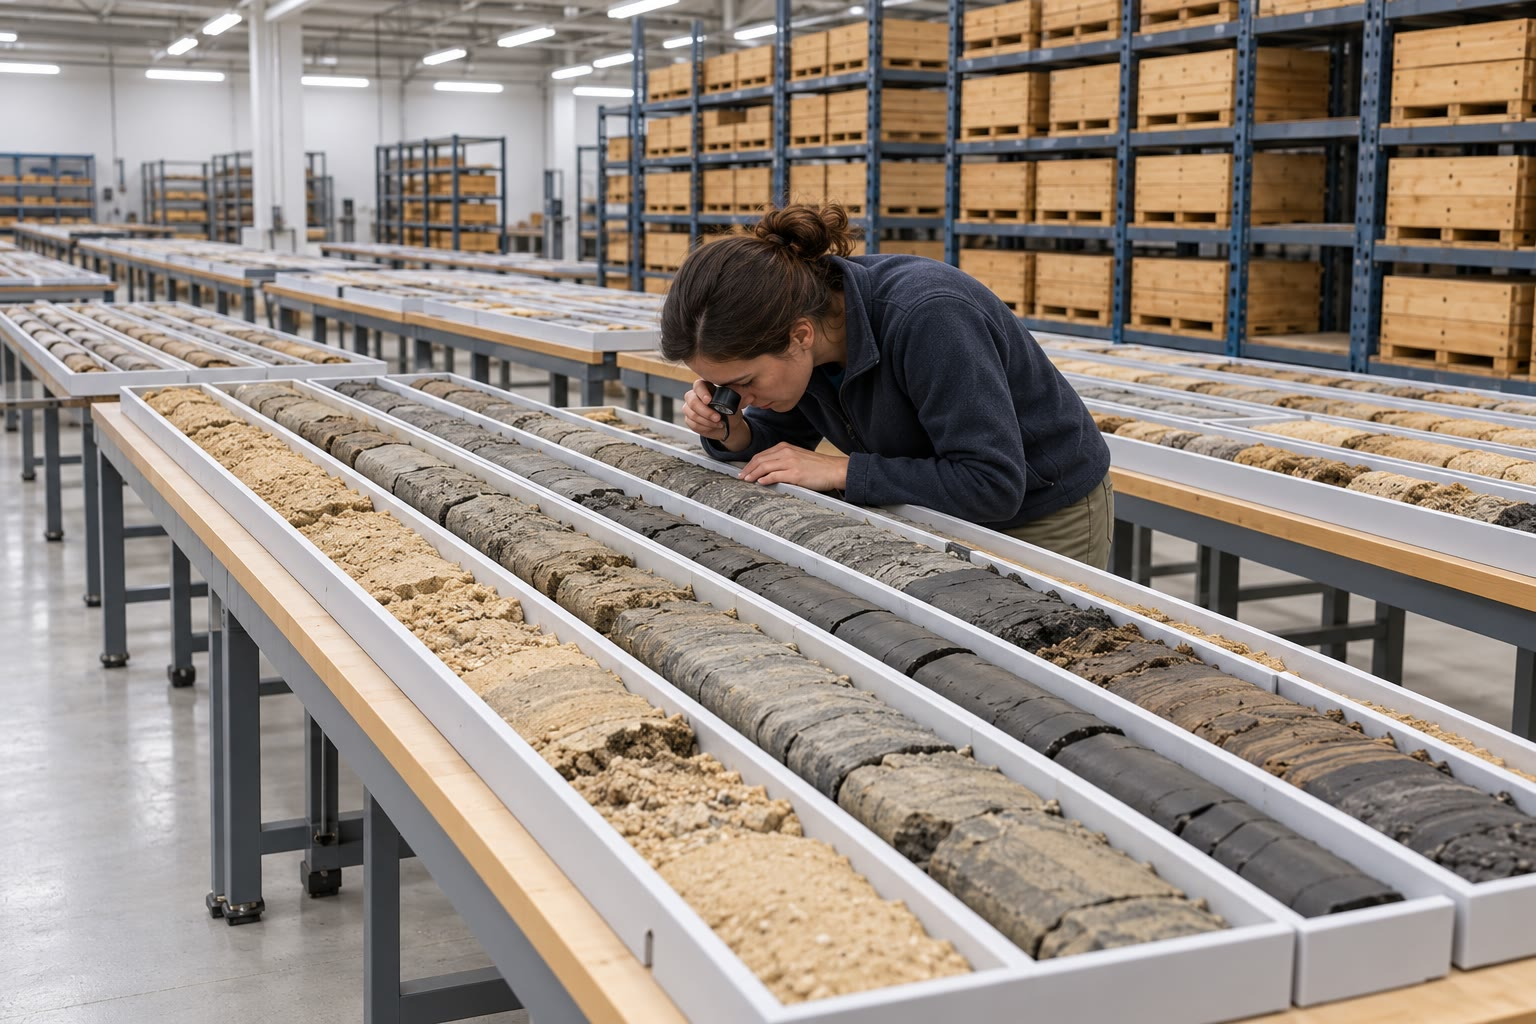
\includegraphics[width=\linewidth]{images/book5/ai/b3-core-store.jpg}

{\scriptsize Un almacén de testigos: testigos partidos de arena y lodo en bandejas, un geólogo
con una lupa de mano. Ilustración generada por IA.}
\end{minipage}
\end{inthelab}

\section{Ejercicios}

\begin{exercise}[$\star$]\label{exo:b3:facies-models:1}
Un testigo muestra, desde la base hacia arriba: lodo de plataforma externa, lodo y arena fina
intercalados, arena de \omterm{def:b3:facies-models:shoreface}{anteplaya}, arena de playa y, después, carbón con raíces. Utilícese la ley de Walther
para dar el orden de los ambientes a lo largo de la costa en ese momento y la dirección
en la que se desplazó la línea de costa. ¿Qué habría dejado una transgresión?
\end{exercise}

\begin{exercise}[$\star$]\label{exo:b3:facies-models:2}
Tres cuerpos de arena presentan formas de rayos gamma: (a) una campana de \qty{8}{m} de espesor con una
base neta; (b) un embudo de \qty{20}{m} de espesor; (c) un cilindro de \qty{30}{m}
de espesor con techo y base netos. Propóngase un ambiente para cada uno y la
observación en un testigo que lo confirmaría.
\end{exercise}

\begin{exercise}[$\star$]\label{exo:b3:facies-models:3}
Una arenisca da $\rho_b = \qty{2.40}{g/cm^3}$. Calcúlese su porosidad con matriz de cuarzo y agua dulce,
y luego con salmuera de \qty{1.1}{g/cm^3}.
\end{exercise}
% ledger: keys:density-porosity

\begin{exercise}[$\star$]\label{exo:b3:facies-models:4}
Olas de longitud de onda modal \qty{75}{m} y \qty{110}{m} (el mar resguardado y el mar abierto del
estudio con boyas). Estímese la profundidad a la que cada una conserva el
\qty{4}{\percent} de su movimiento superficial, y la fracción que queda a una profundidad de
\qty{20}{m}.
\end{exercise}
% ledger: losspeters10:wavebase

\begin{exercise}[$\star\star$]\label{exo:b3:facies-models:5}
Una caliza da $\Delta t = \qty{60}{\micro\second/ft}$. Calcúlese su porosidad con la
ecuación del promedio temporal para una matriz de 47.6 y de
\qty{52.6}{\micro\second/ft}, y salmuera a \qty{189}{\micro\second/ft}. ¿Qué
enseña la diferencia?
\end{exercise}
% ledger: keys:sonic

\begin{exercise}[$\star\star$]\label{exo:b3:facies-models:6}
Un intervalo de \qty{40}{m} contiene capas de arena de 6.0, 3.5, 8.0 y \qty{2.5}{m}
por debajo del límite de corte; el resto es lodo. Calcúlese su \omterm{def:b3:facies-models:ntg}{razón neto--bruto}. Con una
porosidad de \qty{22}{\percent} en la arena, ¿cuánto volumen de poros contiene un kilómetro
cuadrado del intervalo?
\end{exercise}

\begin{exercise}[$\star\star$]\label{exo:b3:facies-models:7}
Una capa de turbidita cerca de la desembocadura de un cañón tiene \qty{1.2}{m} de arena masiva
(Ta) erosionada en la parte superior por la capa siguiente; a \qty{30}{km} aguas abajo del abanico, una capa del
mismo flujo es \qty{8}{cm} de arena fina y limo con laminación de rizos, bajo \qty{3}{cm} de lodo.
Nómbrense las divisiones de cada una y explíquese el cambio.
\end{exercise}

\begin{exercise}[$\star\star$]\label{exo:b3:facies-models:8}
Una \omterm{def:b3:facies-models:association}{sucesión granodecreciente} de \qty{9}{m} de espesor tiene una base neta con guijarros,
arena con estratificación cruzada, arena fina con rizos y lodo con raíces. Interprétese y
estímese la profundidad del canal que la construyó. ¿Puede aplicarse la ley de Walther a través
de su base? ¿Por qué?
\end{exercise}

\begin{exercise}[$\star\star$]\label{exo:b3:facies-models:9}
Un fondo de plataforma desciende \qty{60}{m} en \qty{40}{km}; otro mantiene una profundidad de
\qty{5}{m} durante \qty{30}{km} y luego desciende \qty{300}{m} en
\qty{1.5}{km}. Calcúlense ambos gradientes, nómbrese cada plataforma y las facies esperadas en
el borde de la segunda.
\end{exercise}

\begin{exercise}[$\star\star\star$]\label{exo:b3:facies-models:10}
Una línea de costa prograda a una velocidad $v$ mientras el nivel relativo del mar sube a una
tasa $A$, y su cinturón de \omterm{def:b3:facies-models:shoreface}{anteplaya} tiene una anchura $w$. Muéstrese que la arena de \omterm{def:b3:facies-models:shoreface}{anteplaya}
de la sucesión vertical tiene un espesor $h = wA/v$. Calcúlese para $w = \qty{2}{km}$,
$A = \qty{0.2}{m/kyr}$ y $v = \qty{20}{m/kyr}$, y dígase qué ocurre cuando
$A = 0$. Compárese con la proposición sobre la \omterm{def:b3:sequence-stratigraphy:trajectory}{trayectoria de la línea de costa} del
Capítulo~\ref{ch:b3:sequence-stratigraphy}.
\end{exercise}

\begin{exercise}[$\star\star\star$]\label{exo:b3:facies-models:11}
Una arenisca da $\rho_b = \qty{2.30}{g/cm^3}$ y $\Delta t =
\qty{86}{\micro\second/ft}$. Calcúlese su porosidad a partir de cada registro con una
matriz de arenisca de cuarzo (2.65, \qty{52.6}{\micro\second/ft}) y salmuera (1.0 para la
densidad, \qty{189}{\micro\second/ft}). Si la porosidad sónica es correcta, ¿qué
densidad de grano implica el \omterm{def:b3:facies-models:wireline}{registro de densidad}, y qué podría ser el cemento?
\end{exercise}
% ledger: keys:density-porosity, keys:sonic

\begin{exercise}[$\star\star\star$]\label{exo:b3:facies-models:12}
En un testigo, lodo marino negro descansa directamente sobre un carbón con raíces, con una
delgada capa de restos de conchas en el contacto. Explíquese por qué la ley de Walther no
se aplica a través de él, qué superficie es y cuánta parte de la sucesión costera
puede faltar si el oleaje erosionó el fondo hasta un \omterm{def:b3:facies-models:shoreface}{nivel de base del oleaje de buen tiempo}
de unos \qty{10}{m} al pasar la línea de costa.
\end{exercise}

\section{Problema: Varden-2, un pozo a través de la cobertera}

\begin{problem}[{Problema de fin de semana --- los registros, la porosidad, las facies y la arena neta
de un pozo inventado en el sinclinal de Varden}]
\label{pb:b3:facies-models:1}
El pozo Varden-2 se perfora en el sinclinal de las colinas de Varden, en
(7500, 7000) de la cuadrícula regional, desde una cota del terreno de
\qty{441.0}{m}, hasta una profundidad total de \qty{1200}{m}. Sus registros se dibujan en la
figura de la última sección. Úsense densidades de grano de 2.65 (cuarzo) y
\qty{2.71}{g/cm^3} (calcita), un agua de poro de \qty{1.0}{g/cm^3}, tiempos de tránsito de la matriz,
de 52.6 (arenisca) y \qty{47.6}{\micro\second/ft}
(caliza), y \qty{189}{\micro\second/ft} para el agua.

\medskip\noindent\textbf{Parte I --- Lectura de los registros.}
\begin{enumerate}
\item El \omterm{def:b3:facies-models:wireline}{registro de rayos gamma} salta de 12 a \qty{110}{API} a \qty{766}{m}, desciende
  a 18 a \qty{866}{m}, se vuelve irregular desde \qty{1046}{m} y se estabiliza en
  \qty{85}{API} desde \qty{1166}{m}. Nómbrense las unidades atravesadas, a partir de sus registros.
\item Calcúlese el espesor de cada unidad de la cobertera y la cota de
  la base de la cobertera.
\item La creta da \qty{2.03}{g/cm^3} cerca de la superficie y
  \qty{2.36}{g/cm^3} a \qty{750}{m}. Calcúlese su porosidad a ambas profundidades.
  ¿Qué le ocurre a la creta con la profundidad?
\item ¿Por qué no se asigna una porosidad a la lutita a partir de su densidad?
\item El esquisto da \qty{2.75}{g/cm^3} y \qty{50}{\micro\second/ft}.
  ¿Qué le indica al perforador el basamento rápido, denso y no poroso?
\end{enumerate}

\medskip\noindent\textbf{Parte II --- Porosidad.}
\begin{enumerate}[resume]
\item La caliza da \qty{2.573}{g/cm^3}: calcúlese su porosidad por densidad.
\item Da \qty{58.9}{\micro\second/ft}: calcúlese su porosidad sónica y
  compárese.
\item La arena limpia de los rellenos de canal da \qty{2.32}{g/cm^3}: calcúlese
  su porosidad.
\item Compruébese con su tiempo de tránsito, \qty{79.9}{\micro\second/ft}.
\item Si el agua de poro fuera una salmuera de \qty{1.1}{g/cm^3}, ¿en cuánto cambiaría
  la porosidad por densidad de la arena?
\item ¿Qué unidad sería el mejor acuífero o yacimiento, y cuál sería el
  sello situado encima de él?
\end{enumerate}

\medskip\noindent\textbf{Parte III --- Facies.} Un testigo extraído de 1108 a
\qty{1124}{m} muestra, desde la base: una superficie erosiva con clastos de lodo y
cantos; \qty{10.4}{m} de arena media con estratificación cruzada; \qty{3.2}{m} de arena fina con rizos
que pasa a limo; \qty{2.4}{m} de lodo pardo rojizo con trazas de raíces.
\begin{enumerate}[resume]
\item Dibújese la forma del \omterm{def:b3:facies-models:wireline}{registro de rayos gamma} esperada a lo largo del intervalo testificado.
\item Nómbrense la sucesión y el ambiente de depósito de cada parte.
\item Con la ley de Walther, descríbanse los ambientes que se disponían lado a lado.
\item Estímese la profundidad del canal.
\item La arenisca contiene once unidades de este tipo, cada una sobre una base neta. ¿Qué
  indica el apilamiento acerca del río y de su llanura de inundación?
\item ¿Puede aplicarse la ley de Walther para pasar de una unidad a la siguiente? ¿Por qué?
\end{enumerate}

\medskip\noindent\textbf{Parte IV --- Arena neta.} Los once rellenos de canal,
desde la base de la arenisca, tienen espesores de 14, 9, 12, 7, 16, 10, 13, 8, 11, 12 y
\qty{8}{m}. Cada uno empieza con arena limpia (\qty{30}{API}) sobre una fracción
de su espesor de 0.60, 0.45, 0.55, 0.30, 0.65, 0.40, 0.55, 0.35, 0.50,
0.45 y 0.30, y luego se hace granodecreciente sobre una fracción de 0.25, 0.30, 0.25, 0.40,
0.20, 0.30, 0.25, 0.35, 0.25, 0.30 y 0.35, subiendo el \omterm{def:b3:facies-models:wireline}{registro de rayos gamma} linealmente hasta
\qty{105}{API}, y termina en lodo.
\begin{enumerate}[resume]
\item ¿Qué fracción de cada intervalo granodecreciente queda por debajo del
  corte de \qty{60}{API}?
\item Calcúlese la arena neta de la unidad más baja y de la más gruesa.
\item Calcúlense el total de arena limpia y el total de los intervalos granodecrecientes de la
  arenisca.
\item Calcúlese su \omterm{def:b3:facies-models:ntg}{razón neto--bruto}.
\item ¿Cómo cambiaría la arena neta con un corte de 45 o de
  \qty{75}{API}?
\item Con la porosidad de la arena de la pregunta 8, calcúlese el volumen de poros de la
  arena neta bajo un kilómetro cuadrado.
\item Indíquese el espesor de arena neta de la arenisca triásica de Varden-2.
\end{enumerate}
\end{problem}
% ledger: keys:density-porosity, keys:sonic, keys:gamma
